\chapter{Il cifrario simmetrico standard}

\section{Criteri di Shannon}

\begin{itemize}
    \item \textbf{Diffusione} : Permutazioni ed espansioni del messaggio
    \item \textbf{Confusione} : Combinazione e compressione dei bit del messaggio e e della chiave
\end{itemize}

\section{Il cifrario DES}

\begin{itemize}
    \item Il messaggio viene diviso in blocchi da 64 bit
    \item La chiave \'e composta da 8 Byte in cui ogni ottavo bit \'e di parit\'a
    \item La cifratura e decifrazione del messaggio avviene attraverso 16 round
    \item Dalla chiave vengono create 16 sottochiavi $k[0],k[1],\dots,k[15]$ dette chiavi locali
    \item La decifrazione si esegue invertendo l'ordine delle chiavi locali
    \item Tutte le operazioni del DES sono lineari ad eccezione della S-Box
    \item Tutte le espansioni e compressioni del DES sono progettate in modo e maniera da garantire l'utilizzo di tutti i bit della chiave
\end{itemize}

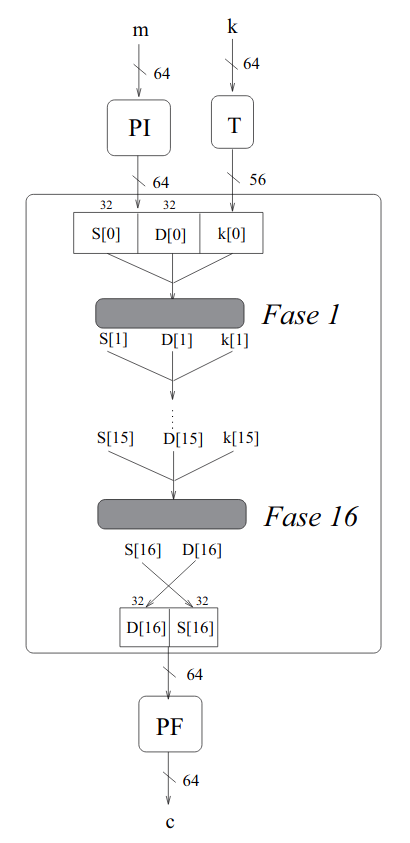
\includegraphics[width=120pt]{des1}
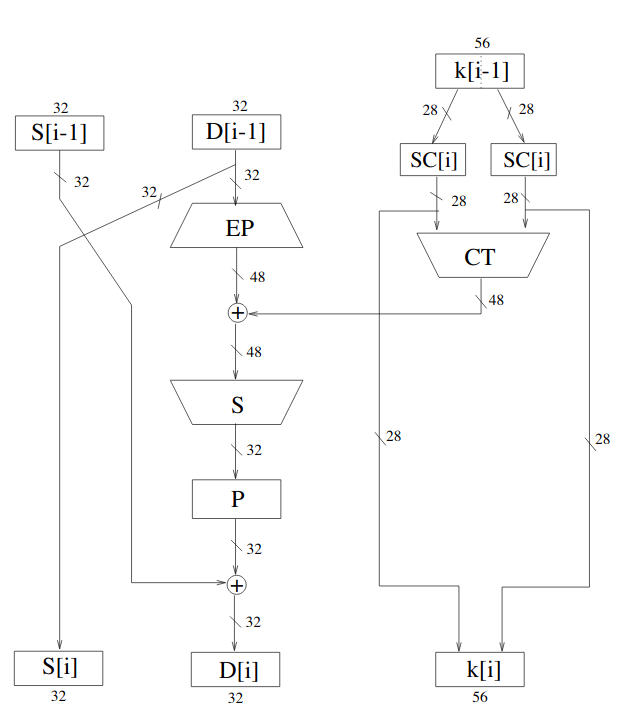
\includegraphics[width=212pt]{des2}

\subsection{Attacchi}
\begin{itemize}
    \item Propriet\'a del complemento
    \begin{itemize}
        \item $\mathcal{C}_{DES}(m, k) = c \implies \mathcal{C}_{DES}(\overline{m}, \overline{k}) = \overline{c}$
        \item Procurandosi alcune coppie $\langle m, c_1 \rangle$ e $\langle \overline{m}, c_2 \rangle$ si pu\`o effettivamente dimezzare il numero di chiavi da testare per un attacco esaustivo
        \item Infatti se testando una chiave $k$ risulta $\mathcal{C}_{DES}(m, k) = c_1$ allora $k$ probabilmente \'e la chiave
        \item Se invece risulta che  $\mathcal{C}_{DES}(m, k) = \overline{c_2}$ allora la chiave potrebbe essere $\overline{k}$
    \end{itemize}
    \item Crittoanalisi differenziale
    \begin{itemize}
        \item Si supponga di riuscire ad ottenere $2^{47}$ coppie $\langle m, c$ con $m$ scelti dal crittoanalista
        \item Si possono quindi analizzare i crittogrammi ottenuti per assegnare probabilit\'a diverse a varie chiavi
        \item La chiave originale dovrebbe quindi emergere come quella con probabilit\'a pi\'u alta
    \end{itemize}
    \newpage
    \item Crittoanalisi lineare
    \begin{itemize}
        \item Date $2^{43}$ coppie $\langle m, c \rangle$ si possono inferire alcuni bit della chiave tramite un'approssimazione lineare della funzione di cifratura e di ricavare gli altri tramite attacco esauriente
    \end{itemize}
\end{itemize}

\subsection{Variazioni del DES}

\begin{itemize}
    \item \textbf{Scelta indipendente delle sottochiavi} : Cio porta la lunghezza della chiave da 56 a 768 bit. In questo caso un attacco con analisi differenziale richiede $2^61$ coppie messaggio crittogramma
\item \textbf{3TDEA} : Si scelgono due chiavi $k_1, k_2$ e si procede come \\$\mathcal{C}_{DES}(\mathcal{D}_{DES}(\mathcal{C}_{DES}(c, k_1), k_2), k_3)$
\item \textbf{2TDEA} : Come 3TDEA con $k_3 = k_1$
\end{itemize}

\section{AES}

\begin{itemize}
    \item Cifrario simmetrico
    \item Il messaggio \'e diviso in blocchi da 128 bit
    \item Le chiavi sono da 128, 192 o 256 bit
    \item In base alla lunghezza della chiave il processo viene iterato 10 (128bit), 12 (192bit), o 14 (256bit) volte
    \item Le operazioni di ogni fase sono:
    \begin{itemize}
        \item \textbf{Op1} : Ogni Byte della matrice B \'e trasformato tramite una S-Box
        \item \textbf{Op2} : La matrice ottenuta \'e permutata tramite shift ciclici sulle righe
        \item \textbf{Op3} : Le colonne risultanti vengono trasformate tramite una operazione algebrica
        \item \textbf{Op4} : Ogni byte della matrice viene messo in \texttt{XOR} con un Byte della chiave locale per quella fase
    \end{itemize}
\end{itemize}

\section{Cifrari a composizione di blocchi}

\begin{itemize}
    \item Per la struttura dei cifrari appena descritti, blocchi identici del messaggio vengono trasformati in blocchi identici del crittogramma.
    \item Per ovviare a questo problema ci si pu\'o affidare ai cifrari a composizione di blocchi
    \item Il messaggio viene diviso in blocchi $m = m_1m_2\dots m_s$ di $b$ bit
    \item Se $m_s$ contiene $r < b$ bit lo si completa aggiungendo la sequenza $10000\dots$ di lunghezza $b - r$, altrimenti si aggiunge un nuovo blocco $m_{s+1} = 10000$
    \item Sia $c_0$ una sequenza di $b$ bit scelta in modo casuale
    \item Allora $c_i = \mathcal{C}(m_i \oplus c_{i-1}, k)$ e $m_i = c_{i-1} \oplus \mathcal{D}(c_i, k)$
\end{itemize}